\documentclass[12pt,letterpaper,noanswers]{exam}
\usepackage[usenames,dvipsnames,svgnames,table]{xcolor}
\usepackage[margin=0.9in]{geometry}
\renewcommand{\familydefault}{\sfdefault}
\usepackage{multicol}
\usepackage{wrapfig}
\pagestyle{head}
\definecolor{c03}{HTML}{FFDDDD}
\header{AM 22b Class 19}{}{Mar 15: Vector fields}
\runningheadrule
\headrule
\usepackage{graphicx} % more modern
\usepackage{amsmath} 
\usepackage{amssymb} 
\usepackage{hyperref}
\usepackage{tcolorbox}
\usepackage[utf8]{inputenc}
\pagenumbering{arabic}

\usepackage[numbered,autolinebreaks,useliterate]{mcode}

\newcommand{\mb}[1]{\underline{#1}}

\begin{document}
 \pdfpageheight 11in 
  \pdfpagewidth 8.5in




% I need to review the torus trajectories...

\begin{itemize}
% \item There is a pre-class assignment (20 minutes of videos + a few WeBWorK exercises) due at 10am this Monday.  It is available on Canvas.
\itemsep0em
      \item The next skill check will be for C19, C20, C21 on Monday Mar 22nd.
    \item There is a pre-class assignment for Wed Mar 17th.
    \item There is a discussion board post due Thurs Mar 18th (no problem set).
    \item Quiz 03 will be posted on Friday Mar 19th (info is on Canvas).
    \item There are no office hours this Tuesday (wellness day).
\end{itemize}

\hrule
\vspace{0.2cm}

\noindent\textbf{Skill Check C19 Practice}
\begin{questions}
\question Assume $x,y>0$.  For $\mb F = x\mb j$, decide if
\begin{parts}
\item the vectors in the vector field are

\begin{oneparcheckboxes}
\choice parallel to the $x$-axis
\choice parallel to the $y$-axis
\choice neither
\end{oneparcheckboxes}
\part As $x$ increases the length of the vectors

\begin{oneparcheckboxes}
\choice increases
\choice decreases
\choice neither
\end{oneparcheckboxes}

\part As $y$ increases the length of the vectors

\begin{oneparcheckboxes}
\choice increases
\choice decreases
\choice neither
\end{oneparcheckboxes}
\end{parts}
\end{questions}


\vspace{0.2cm}
\hrule
\vspace{0.2cm}

\noindent\textbf{Skill Check C19 Practice Solution}
\begin{questions}
\question 
\begin{parts}
\item The vector field is $\langle 0, x\rangle$ so vectors are parallel to the $y$-axis.
\item As $x$ increases $\Vert \mb F \Vert = \vert x \vert$ also increases.
\item As $y$ increases $\Vert \mb F \Vert = \vert x \vert$ does not change, so neither increases nor decreases.
\end{parts}
\end{questions}

\vspace{0.2cm}
\hrule
\vspace{0.2cm}


% partial derivatives, gradient
% local linearity, differential, directional deriv
% 2nd order partials + equations with partials

\noindent\textbf{Big picture}

Today is focused on vector valued functions, today interpreted as vector fields rather than as parameterized curves or surfaces.  We will soon return to integration (with these new functions).

\vspace{0.2cm}
\hrule
\vspace{0.2cm}

\noindent\textbf{Teams}

You will work with this team on the in-class problems today.
\begin{multicols}{2}
1.  student names

\end{multicols}

%\vspace{0.2cm}
\hrule
\vspace{0.2cm}

\eject

\vspace{0.2cm}
\hrule
\vspace{0.2cm}

\noindent\textbf{Vector fields} \S 17.3

\begin{tcolorbox}
 A function $f: \mathbb{R}^n \rightarrow \mathbb{R}^k$ is a \textbf{vector-valued function} because there are multiple outputs associated with each input.  
    
    The output of the function can be interpreted in two different ways: 
    \begin{itemize} 
    \itemsep0em
    \item as a mapping assigning a vector in $k$-space to each point in $\mathbb{R}^n$.  This is a \textbf{vector field}
    \item as a mapping assigning a point in $k$-space to each point in $n$-space.  This is a \textbf{parameterization}.
    \end{itemize}
    
To create a representation of a vector field, 
\begin{itemize}
    \itemsep0em
\item we sketch vectors at points in $\mathbb{R}^n$.  
\item Although we only draw the vectors at select points, the
vector field is defined for every point in the domain. \\
\end{itemize}
\end{tcolorbox}



\noindent\textbf{Example (vector field)}.  
\begin{multicols}{2}
Consider
$\mb F(x,y) = x\mb i + 0 \mb j.$  At each point $(x,y)$ in the $xy$-plane we have a corresponding vector $x\mb i$.  We can sketch these vectors.  This is the vector field $\mb F(x,y) = \langle x,0\rangle$.



Sketch this vector field using a unit grid ranging from $-2\leq x \leq 2$, $2\leq y\leq 2$.

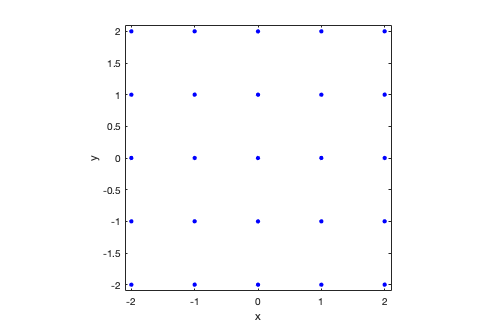
\includegraphics[width=3in]{img/C17grid.png}
\end{multicols}

\noindent\textbf{Question (matching)}.  Match the vector fields \[f(x)\mb i, \quad g(x)\mb j, \quad h(y)\mb i,\quad k(y)\mb j\] to the images below.  %\emph{pollQ}.

\hspace{-0.5in}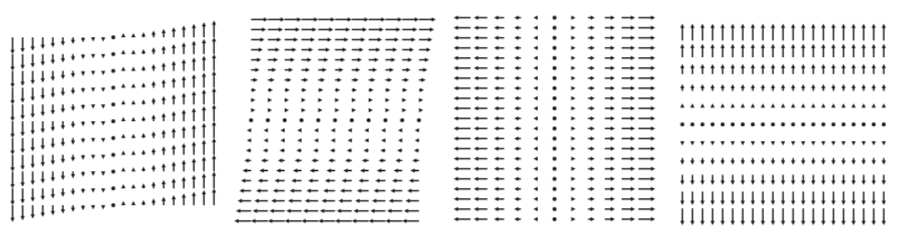
\includegraphics[width=\linewidth]{img/C24p2b-18.png}
\vfill
%

\noindent\textbf{Question (matching)}.  Match the vector fields \[f(x)\mb i+f(x)\mb j,\quad g(x)\mb i - g(x)\mb j,\quad h(y)\mb i + h(y)\mb j,\quad k(y)\mb i - k(y)\mb j\] to the images below. % \emph{pollQ}.

\hspace{-0.5in}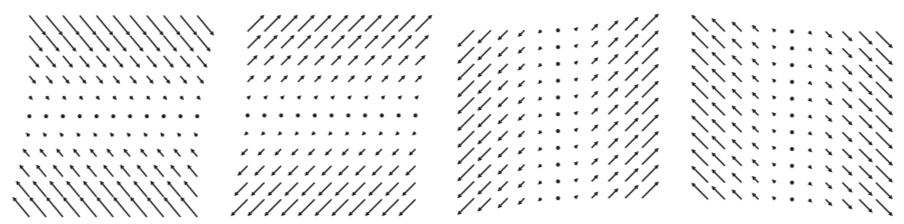
\includegraphics[width=\linewidth]{img/C24p3b-18.png}

\vfill


\noindent\textbf{Examples (vector fields to know)}. 

$\mb F_i = \mb r$, $\mb F_{ii} = \frac{\mb r}{\Vert \mb r\Vert}$.  $\mb F_{iii} = x\mb j$.  $\mb F_{iv} = y\mb i - x\mb j.$


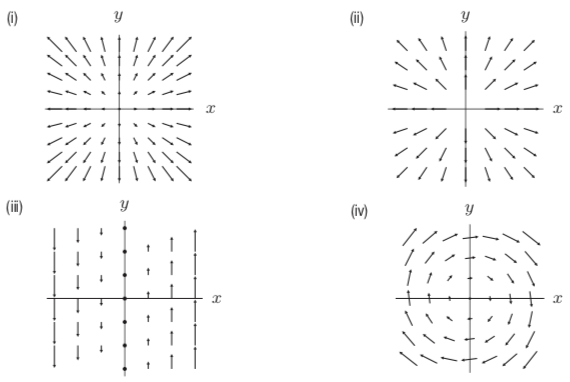
\includegraphics[width=0.8\linewidth]{img/C24p4-18.png}

\vfill




\vspace{0.2cm}
\hrule
\vspace{0.2cm}

\begin{tcolorbox}


\noindent\textbf{Force fields} are a common type of vector field.  Because forces have a direction as well as a magnitude, and force fields act at each point in space, a vector field is an appropriate representation. 
\end{tcolorbox}

Below is a visualization of a magnetic field.  The vectors themselves are not quite visible.  Each iron filing is aligned with the magnetic field.  However the length of filings does not vary with the strength of the field, as it would it we were drawing in vectors:

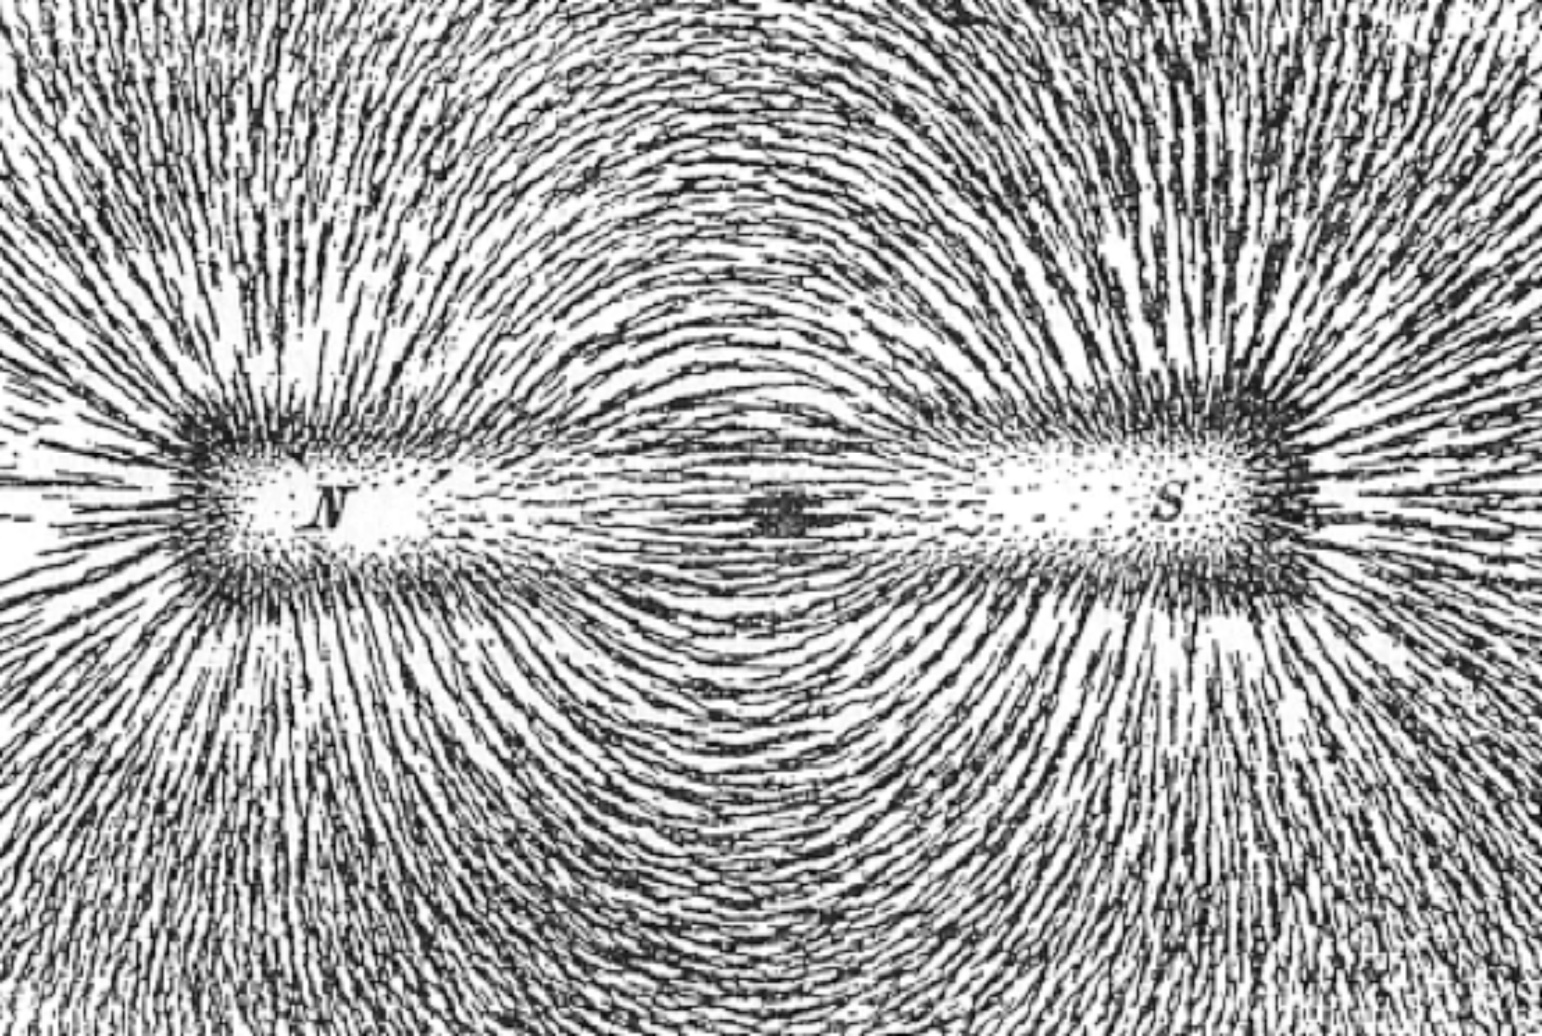
\includegraphics[width=3in]{img/C24p5.png}

\url{http://www.txessrevolution.org/MagneticSun_Info}

\vspace{0.1cm}

\noindent\textbf{Example: gravitational force}

$\displaystyle\mb F(\mb r) = -\frac{GMm\mb r}{\Vert \mb r\Vert^3}$.  $\mb r = \langle x, y, z\rangle$, so this is a compact notation for
$\displaystyle\mb F(\mb r) = -GMm(\frac{x}{(x^2+y^2+z^2)^{3/2}}\mb i+\frac{y}{(x^2+y^2+z^2)^{3/2}}\mb j + \frac{z}{(x^2+y^2+z^2)^{3/2}}\mb k$
 
$\mb F(\mb r)$ is a radial vector field where all vectors point towards the origin.
 

\includegraphics{img/N24_p4.pdf}

\vspace{0.1cm}

\noindent\textbf{Example (dolphin motion)}.
Velocity vectors of the water motion as a dolphin swims are shown (with their length indicated by color) at nine different timepoints.

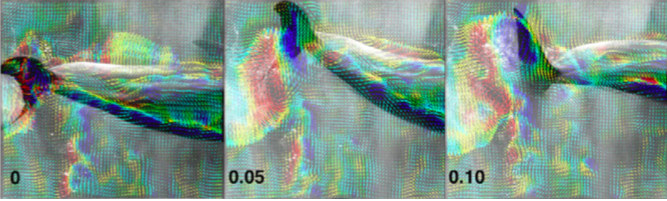
\includegraphics[width=0.8\linewidth]{img/C24p1b-18.png}

\cite{fish2014measurement}
\vfill




\noindent\textbf{Example (wind velocity)}.

Here is an example where vectors are indicating the wind velocity near Hurricane Katrina (measured by a satellite in Aug 2005):

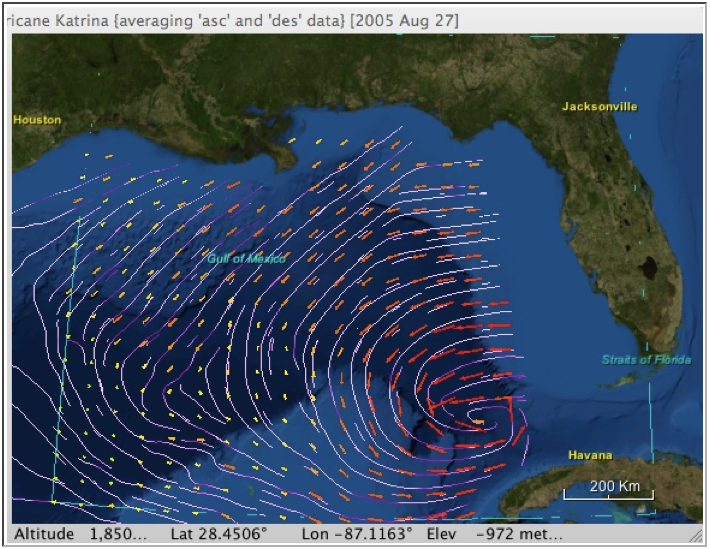
\includegraphics[width=5in]{img/N24_p2.png}

\url{https://people.eecs.ku.edu/~miller/WorldWindProjects/VectorFieldVis/5DayKatrinaNoGrid.html}



The length of each vector indicates its relative magnitude.  The vectors are color coded by magnitude: red is high speed, and yellow low.  


\vspace{0.2cm}
\hrule
\vspace{0.2cm}

\noindent\textbf{Velocity vector fields: flow lines} \S 17.4
\begin{tcolorbox}
  A \emph{flow line} of a vector field $\mb v = \mb F(\mb r)$ is a path $\mb r(t)$ where the velocity vector at each point on the path is equal to $\mb v$.  On a flow line $\frac{d\mb r}{dt}(t) = \mb v = \mb F(\mb r(t))$. \\

The \emph{flow} of a vector field is the family of all of its flow lines.

\tcblower

The lines superimposed on the image of wind velocities are flow lines (sometimes called \emph{stream lines}).  They indicate the trajectory a massless tracer particle would follow if it were subjected to these wind velocities. \\

It is common to visualize a vector field using flowlines (streamlines).
\end{tcolorbox}


\noindent\textbf{Flow lines}.  Match each of $\mb F_1 = -y\mb i + x\mb j$, $\mb F_2 = x\mb i - y\mb j$ and $\mb F_3 = y\mb i + x\mb j$ to a vector field and to a plot of flow lines below.

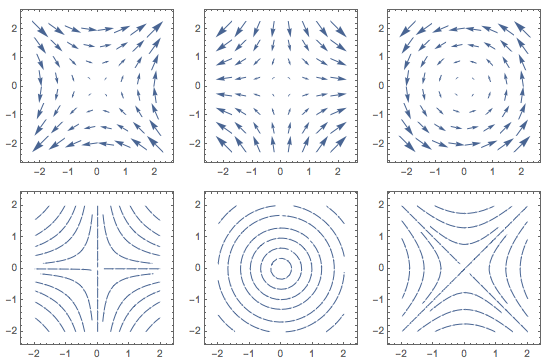
\includegraphics[width=0.9\linewidth]{img/C24p6-18.png}

\vfill





\noindent\textbf{Example (today's wind)}.

Flow lines are found by seeding a region with tracer particles and seeing how they travel under the action of the vector field (where vectors are treated as velocities).  Below is a snapshot of a visualization of wind at the surface of the earth in the North Atlantic on the morning of this class.

% \includegraphics[width=5in]{N24_p3.png}  % October 28th 2016

%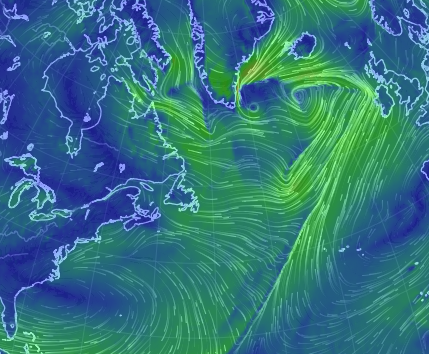
\includegraphics[width=3in]{img/C17todaywind.png}
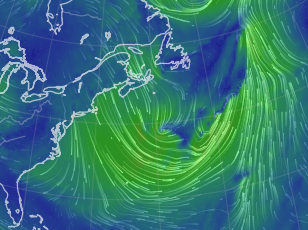
\includegraphics[width=3in]{img/C19-wind.png}

\url{https://earth.nullschool.net/#current/wind/surface/level/orthographic=-64.86,47.01,444}

\vspace{0.2cm}
\hrule
\vspace{0.2cm}



\bibliographystyle{plainnat}
\bibliography{main}

\end{document}